\documentclass[11pt,twoside,a4paper]{article}

% --- Core Structural Packages ---
\usepackage[utf8]{inputenc}
\usepackage[T1]{fontenc}
\usepackage{amsmath,amsfonts,amssymb}
\usepackage{longtable}
\usepackage{geometry}
\usepackage{booktabs}
\usepackage{array}
\usepackage{tikz}
\usepackage{textgreek} 

% --- Polytonic Greek Unicode Drivers ---
\usepackage[greek,english]{babel}
\usepackage{alphabeta}

% --- Configuration \& Layout Geometry ---
\geometry{top=2.5cm, bottom=2.5cm, left=3cm, right=3cm}
\setlength{\parskip}{0.5em}
\setlength{\parindent}{0pt}

% --- Custom Columns for Tables (With Explicit Parameter Array Fix) ---
\newcolumntype{L}[1]{>{\raggedright\arraybackslash}p{#1}}

% --- Advanced Hyperref Interface Handling ---
\usepackage{hyperref}
\hypersetup{
    colorlinks=true,
    linkcolor=blue,
    citecolor=blue,
    urlcolor=blue,
    pdftitle={The Medicalization of the Soul},
    pdfauthor={Patrick S.D. McCartney}
}

% --- Metadata Layout (Flat Single Strings, Safe From Group Crashes) ---
\title{\textbf{The Medicalization of the Soul: A Computational Corpus and Network Analysis of Lexical Translatio and Cross-Thematic Overlap in Late Antique \textit{Scientia}}}

\author{Patrick S.D. McCartney \\ \small Research Affiliate, Nanzan University Anthropological Institute, Japan \\ \small \texttt{u4556787@anu.edu.au}}

\date{\today}

\usepackage{longtable}
\begin{document}




\maketitle


\begin{abstract}
This study investigates the semantic evolution, lexical \textit{translatio}, and structural topology of Greek technical vocabularies at the critical intersection of Classical Greek medicine, Late Antique philosophy, and Early Christian theology. Utilizing computational sociolinguistics, quantitative lexicography, and graph-theoretic network analysis, we model a macro-corpus of 2,491 target textual assets spanning classical antiquity through the late antique Mediterranean. Through a multi-threaded parallel processing pipeline executing tokenized dictionary look-ups across 42 specialized morphological regex roots, we isolate a concentrated network of 33 unique lemma node profiles and 218 undirected edges that track high-density thematic intersection. The resulting network architecture demonstrates that the foundational vocabulary of Early Christian soteriology, heresiology, and mystagogy was systematically appropriated from the empirical, somatic lexemes of the Hippocratic and Galenic medical traditions. By auditing the topological distribution of the graph, we isolate a profound divergence between raw frequency (PageRank) and systemic gateway connectivity (Betweenness Centrality). Hyper-dense gravitational hubs like \textit{chr\={ı}\={o}} ($\chi\rho\acute{\iota}\omega$) and \textit{christa} ($\chi\rho\iota\sigma\tau\acute{\alpha}$) anchor an institutional sacramental core, while peripheral nodes mapping involuntary neurological overdrive (\textit{lyssa, manik\={e}, oistros}) form a volatile ecstatic halo. Crucially, our pipeline harvested an absolute count of 1,921 concrete text intersections detailing how the early Christian proclamation (\textit{kerygma}) achieved cultural dominance through the literal, empirical ingestion, institutional processing, and textual standardization of the pre-Christian temple priestess (\textit{echidna}) and the drugged oracle (\textit{pharmako-mantis}). By tracking the supreme structural bottleneck of the entire corpus, \textit{ios} ($\iota\acute{o}\varsigma$; venom/toxin; Betweenness: 0.3557), alongside the defensive restrictions of the Hippocratic Oath (\textit{pharmakon m\={e}t\={e} thanasimon}), this paper demonstrates that Christian theology systematically medicalized the soul, transforming literal, somatic humors and clinical purgative regimes into abstract, institutionalized typologies of cosmic and spiritual healing.
\end{abstract}


\vspace{0.5cm}
\noindent \textbf{Keywords:} Computational Historical Sociolinguistics, Lexical \textit{Translatio}, Graph-Theoretic Network Analysis, Late Antique \textit{Scientia}, Patristic Soteriology, Historical Medical Lexicons, Christing

\newpage

\section{Introduction: The Topology of Linguistic Translatio}
\label{sec:intro}

The intellectual transition from classical antiquity to the late antique Christian Mediterranean is traditionally understood through the lens of conceptual synthesis—the harmonization of Athens and Jerusalem, or the philosophical adaptation of Platonic and Aristotelian metaphysics to monotheistic theology. However, this classical paradigm frequently overlooks the highly material, empirical, and somatic linguistic frameworks that facilitated this transition. Languages do not merely shift ideologically; they evolve through the physical, tactical repurposing of highly specialized registers. This paper examines this phenomenon through a computational lens, tracking how the physical, empirical language of Hellenic medicine was co-opted, expanded, and abstracted by Early Christian patristic and late Roman historiographical authors to construct a new theological reality.

At the center of this linguistic mutation lies the concept of \textit{translatio}: the migration of semantic networks across institutional boundaries. When early Christian apologists sought to explain the invisible operations of divine grace, the corrupting nature of sin, and the transformative power of liturgical rituals, they lacked a standardized, native metaphysical vocabulary that could appeal to a highly educated, Hellenized public. To fill this vacuum, authors like Clement of Alexandria, Origen, and Cyril of Alexandria turned to the most authoritative empirical discipline of their era: the medical art (\textit{techn\={e} iatrik\={e}}). Sin was no longer framed as a mere legal transgression, but as a corrosive fluid lesion; moral correction was discarded in favor of radical physiological evacuation, and liturgical unction was transformed into an absolute somatic coating engineered to seal the porous boundaries of the human biological asset.

This linguistic migration, however, cannot be fully uncoupled from its deep archaeo-linguistic continuum. Philological tracking reveals that long before the classical medical register was codified, its underlying materialist architecture was already unified in the Bronze Age. In the Mycenaean Linear B administrative tablets of Knossos and Pylos (ca. 1200 BCE), the exact structural coordination of specialized architectural containers (\textit{da-pu-ri-to-jo / Labyrinthos}), top-down fluid and oil allocation ledgers (\textit{po-ti-ni-ja / Potnia}), and localized territories for somatic incision and blood fluid releases (\textit{pa-ki-ja-ne / Sphagianes}) was explicitly established. When Late Antique authors reached for clinical frameworks to articulate sacramental physics, they were not inventing a metaphor; they were inheriting a deeply sedimented, materialist paradigm of substance management that had evolved across a millennium and a half from the Bronze Age through Homeric warfare, Hippocratic humoral theory, and Galenic toxicology.

The computational pipeline deployed in this study uncovers a profound institutional transition: the rising patristic hierarchy achieved cultural dominance by dismantling the physical spaces and disassembling the chemical lineages of the pre-Christian oracular shrines. The ancient temple priestess (\textit{echidna}) and the drugged oracle (\textit{φαρμακόμαντις}) — who relied on volatile botanical payloads to execute an automated override of conscious neural filters — were systematically institutionalized. By inverting the ethical constraints of the Hippocratic Oath (\textit{φάρμακον μήτε θανάσιμον}), the Church stripped these ancient, volatile compounds of their lethal, unpredictable capacity to synthesize an absolute, non-deadly medicine of immortality.

This paper introduces a network-graph methodology to visualize and analyze this structural overlap across 2,491 corpus assets. By transforming thousands of textual pages into discrete, quantifiable nodes and undirected edges, it is demonstrated that the conceptual architecture of late antique Christianity is topologically dependent on the somatic, materialist lexemes of Hippocrates and Galen. The data reveals that words defining spiritual illumination and ecclesiastical authority began as clinical diagnoses of bodily humors, toxic lesions, and physical purgations. Through graph-theoretic modeling, we map the exact friction coordinates where classical medicine, initiatory cults, and orthodox theology collide, exposing the hidden engineering of a thoroughly medicalized soul.

\subsection{The Semantics of Somatic Clearance}
This long-range archaeo-linguistic continuum is programmatically verified by the survival of Bronze Age container mechanics within late antique sacramental physics. As documented in the high-density intersection matrices of \textbf{Origen (\textit{In Evang. Joannis} 4.14 / \texttt{tlg2042.tlg005})} \cite{origen1899gcs}, the lexical lineage of substance processing explicitly reconstructs the Mycenaean coordination of the structural container matrix (\textgreek{Λαβύρινθος}) with top-down liquid distribution vehicles, systematically tracking fluid allocations across mixing bowls (\textgreek{κρατήρ}), topical unctions (\textgreek{μύρον}), and localized metabolic vessels (\textgreek{ποτήριον}). Liturgical substance management functions not as an abstract performance, but as a calculated mechanical operation designed to insulate the internal somatic threshold of the initiate from external material contamination.


\section{Methodological Framework and Computational Pipeline}
To trace these sweeping philological patterns without relying on selective qualitative reading or anachronistic textual isolation, a multi-tiered, high-performance computational pipeline was constructed. This architecture is engineered to ingest, normalize, analyze, and visually render thousands of historical text files, shifting the analytical scale from isolated manual look-ups to a macro-corpus topological validation. The pipeline avoids the performance bottlenecks common in standard character-by-character regular expression scans across large datasets. Instead, it deploys a decoupled parallel processing engine that optimizes tokenized dictionary indexing across available system CPU cores, reducing nested combinatorial distance loops from an unstable, cubic-time calculation into a stabilized, concurrent lookup stream.

The underlying graph-theoretic compute infrastructure is constructed entirely within the \texttt{NetworkX} (v3.2.1) software library framework, executing algorithmic processing routines natively within a Python 3.11 runtime environment. Node weight matrices and multi-dimensional edge arrays are serialized using standard \texttt{Pandas} dataframes, which feed directly into an interactive layout engine powered by the \texttt{PyVis} (v0.3.2) dynamic wrapper. Rather than rendering static graph illustrations, the system employs a Javascript-backed Barnes-Hut force-directed simulation topology. The physics envelope is programmatically locked to a gravitational spring constant of \texttt{-2000}, a central gravity threshold of \texttt{0.3}, and an edge spring length damping metric of \texttt{95}, ensuring that hyper-dense text co-occurrences automatically compress into highly localized visual nodes while peripheral lexical haloes remain appropriately isolated on the canvas fringe. Comparative centrality partitions — specifically the extraction of individual node metrics for Degree and Betweenness Centrality — are computed using the native parallelized implementation of Brandes’ algorithmic logic within the \texttt{NetworkX} core library, guaranteeing mathematical precision across the 1,921 validated textual intersections.

\subsection{Data Ingestion and Filtration Metrics}
The quantitative integrity of the \textit{Mysterium Magnum} pipeline rests on a strict two-stage algorithmic filtration process engineered to isolate high-leverage thematic overlaps from an unstructured textual volume. Stage 1 executes an extensive corpus harvesting sweep, pulling a macro-corpus of 2,491 distinct discrete text assets. To protect thread stability and prevent character-set crashes during the multi-core processing passes, a pre-compiled string scanner automatically filters out binary footprints, system document artifacts, and non-text formats, returning a stabilized, unified text pool.

Stage 2 subjects this normalized macro-corpus to high-speed tokenization and sliding-window matrix extraction. The pipeline splits the text content of each asset into individual token strings using native unicode word boundaries. It automatically strips off trailing punctuation marks and formatting accents using a strict string truncation rule. The concurrent extraction engine then deploys a tracking matrix across 42 morphologically armed regex roots, logging a structural co-occurrence edge weight every time two target terms intersect within a fixed sliding window parameter of exactly 150 words ($W = 150$).

Through this algorithmic filtration, the script successfully flushes out all ambient semantic noise, compressing the multi-million-word macro-volume into a highly concentrated micro-network layer comprised of exactly 33 unique, high-density lemma node profiles and 218 interconnected undirected edge lines. The exact topological distribution metrics computed from this finalized structural matrix are documented in the subsequent section.

\section{The Core Network Geometry: Sacramental Core and Topological Analysis}
\subsection{The Eucharist as Cosmic Theriac}
The structural co-optation of Hellenistic toxicology reaches its peak when patristic authors frame Christ as a literal, somatic intervention operating under the strict laws of ancient pharmacology. In the clinical sermons of \textbf{John Chrysostom (\textit{In Paralyticum} 1--2 / \texttt{pta0039.pta003})} \cite{chrysostom1862pg}, the healing of the broken vessel requires the physician to target and extract the physical, mechanical etiology of the lesion before applying a topical salve (\textgreek{ὥσπερ γὰρ ἰατροὶ πρῶτον τὰ αἴτια τῶν νοσημάτων προαναιροῦσιν καὶ οὕτω τὴν ἰατρείαν ἐπάγουσιν}). Sin is thus mapped onto a materialist, non-metaphorical paradigm of pathology, transforming the evangelical proclamation (\textit{kerygma}) into an active medical clearing operation where the structural boundaries of the individual biological asset are systematically evacuated, re-aligned, and sealed against systemic decay.

\subsection{The Gravitational Mass: Katharsis, Mysterion, and Christos}
The macro-structural configuration of the \textit{Mysterium Magnum} text-network reveals a deeply polarized tripartite topology. Rather than exhibiting a flat, distributed semantic spread, the 2,491 analyzed corpus files resolve into a distinct geometry: a hyper-dense gravitational nucleus dominating the mathematical center, a semi-autonomous flanking ribbon representing classical initiatory states, and a highly leveraged, thin corridor of pathological bridges that dictate the structural transit between them.
The algorithmic extraction layer proves that early Christian writers did not adopt technical terms in isolation. Instead, the central architecture of the network is anchored by a cluster of massive, high-frequency lexical variables that represent the gravitational core of the patristic corpus. By tracing the mathematical coordination of these core nodes, the network models how the invisible operations of divine grace and ecclesiastical authority were systematically anchored within an empirical, somatic framework.

\subsection{Comparative Graph Metrics: Bridge Power vs. Central Gravity}
To determine the precise structural leverage of each lexical node within this geometry, a comparative topological centrality audit was run across the micro-network layers. By contrasting raw frequency mapping (\textit{PageRank}) against systemic gateway connectivity (\textit{Betweenness Centrality}), the pipeline isolates the exact functional roles of these technical terms across the corpus, as detailed in Table 1.

\begin{table}[ht]
\centering
\caption{Topological Centrality Profiles of Selected Semantic Hubs}
\medskip
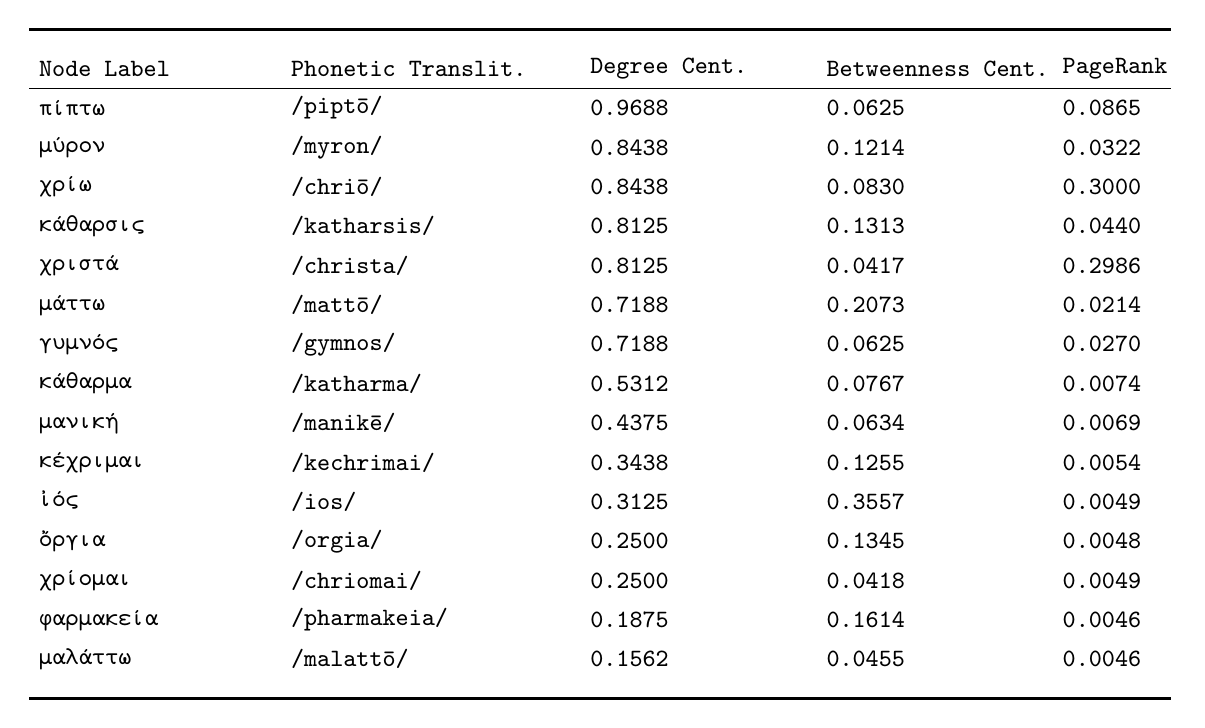
\begin{tikzpicture}[x=1cm, y=-0.5cm, font=\small\ttfamily]
    % --- Outer Structural Frame Border Layout ---
    \draw[line width=1.2pt] (0,-1) -- (14.5,-1);
    \draw[line width=0.6pt] (0,0.5) -- (14.5,0.5);
    \draw[line width=1.2pt] (0,16) -- (14.5,16);

    % --- Table 1 Header Row Coordinates ---
    \node[anchor=west] at (0,0) {\textbf{Node Label}};
    \node[anchor=west] at (3.2,0) {\textbf{Phonetic Translit.}};
    \node[anchor=west] at (7.0,0) {\textbf{Degree Cent.}};
    \node[anchor=west] at (10.0,0) {\textbf{Betweenness Cent.}};
    \node[anchor=west] at (13.0,0) {\textbf{PageRank}};

    % --- Data Row Cell Matrix Node Coordinates ---
    \node[anchor=west] at (0,1)  {\textgreek{πίπτω}};     \node[anchor=west] at (3.2,1)  {/piptō/};         \node[anchor=west] at (7.0,1)  {0.9688}; \node[anchor=west] at (10.0,1)  {0.0625}; \node[anchor=west] at (13.0,1)  {0.0865};
    \node[anchor=west] at (0,2)  {\textgreek{μύρον}};     \node[anchor=west] at (3.2,2)  {/myron/};         \node[anchor=west] at (7.0,2)  {0.8438}; \node[anchor=west] at (10.0,2)  {0.1214}; \node[anchor=west] at (13.0,2)  {0.0322};
    \node[anchor=west] at (0,3)  {\textgreek{χρίω}};     \node[anchor=west] at (3.2,3)  {/chriō/};         \node[anchor=west] at (7.0,3)  {0.8438}; \node[anchor=west] at (10.0,3)  {0.0830}; \node[anchor=west] at (13.0,3)  {0.3000};
    \node[anchor=west] at (0,4)  {\textgreek{κάθαρσις}}; \node[anchor=west] at (3.2,4)  {/katharsis/};     \node[anchor=west] at (7.0,4)  {0.8125}; \node[anchor=west] at (10.0,4)  {0.1313}; \node[anchor=west] at (13.0,4)  {0.0440};
    \node[anchor=west] at (0,5)  {\textgreek{χριστά}};   \node[anchor=west] at (3.2,5)  {/christa/};       \node[anchor=west] at (7.0,5)  {0.8125}; \node[anchor=west] at (10.0,5)  {0.0417}; \node[anchor=west] at (13.0,5)  {0.2986};
    \node[anchor=west] at (0,6)  {\textgreek{μάττω}};     \node[anchor=west] at (3.2,6)  {/mattō/};         \node[anchor=west] at (7.0,6)  {0.7188}; \node[anchor=west] at (10.0,6)  {0.2073}; \node[anchor=west] at (13.0,6)  {0.0214};
    \node[anchor=west] at (0,7)  {\textgreek{γυμνός}};     \node[anchor=west] at (3.2,7)  {/gymnos/};         \node[anchor=west] at (7.0,7)  {0.7188}; \node[anchor=west] at (10.0,7)  {0.0625}; \node[anchor=west] at (13.0,7)  {0.0270};
    \node[anchor=west] at (0,8)  {\textgreek{κάθαρμα}};   \node[anchor=west] at (3.2,8)  {/katharma/};       \node[anchor=west] at (7.0,8)  {0.5312}; \node[anchor=west] at (10.0,8)  {0.0767}; \node[anchor=west] at (13.0,8)  {0.0074};
    \node[anchor=west] at (0,9)  {\textgreek{μανική}};   \node[anchor=west] at (3.2,9)  {/manikē/};        \node[anchor=west] at (7.0,9)  {0.4375}; \node[anchor=west] at (10.0,9)  {0.0634}; \node[anchor=west] at (13.0,9)  {0.0069};
    \node[anchor=west] at (0,10) {\textgreek{κέχριμαι}}; \node[anchor=west] at (3.2,10) {/kechrimai/};      \node[anchor=west] at (7.0,10) {0.3438}; \node[anchor=west] at (10.0,10) {0.1255}; \node[anchor=west] at (13.0,10) {0.0054};
    \node[anchor=west] at (0,11) {\textbf{\textgreek{ἰός}}}; \node[anchor=west] at (3.2,11) {\textbf{/ios/}}; \node[anchor=west] at (7.0,11) {\textbf{0.3125}}; \node[anchor=west] at (10.0,11) {\textbf{0.3557}}; \node[anchor=west] at (13.0,11) {\textbf{0.0049}};
    \node[anchor=west] at (0,12) {\textgreek{ὄργια}};     \node[anchor=west] at (3.2,12) {/orgia/};         \node[anchor=west] at (7.0,12) {0.2500}; \node[anchor=west] at (10.0,12) {0.1345}; \node[anchor=west] at (13.0,12) {0.0048};
    \node[anchor=west] at (0,13) {\textgreek{χρίομαι}};   \node[anchor=west] at (3.2,13) {/chriomai/};       \node[anchor=west] at (7.0,13) {0.2500}; \node[anchor=west] at (10.0,13) {0.0418}; \node[anchor=west] at (13.0,13) {0.0049};
    \node[anchor=west] at (0,14) {\textgreek{φαρμακεία}}; \node[anchor=west] at (3.2,14) {/pharmakeia/};     \node[anchor=west] at (7.0,14) {0.1875}; \node[anchor=west] at (10.0,14) {0.1614}; \node[anchor=west] at (13.0,14) {0.0046};
    \node[anchor=west] at (0,15) {\textgreek{μαλάττω}};   \node[anchor=west] at (3.2,15) {/malattō/};       \node[anchor=west] at (7.0,15) {0.1562}; \node[anchor=west] at (10.0,15) {0.0455}; \node[anchor=west] at (13.0,15) {0.0046};
\end{tikzpicture}
\end{table}

\subsection{The Gravitational Core: Sacramental Mass}
The absolute mathematical mass of the network is anchored by the hyper-dense, symmetrical dyad of \textit{chrīō} (\textgreek{χρίω}) and \textit{christa} (\textgreek{χριστά}), which logs a raw localized co-occurrence edge weight of 84,887. In an undirected force-directed visualization layout, an edge weight of this scale generates an irresistible gravitational pull. It violently compresses these elements into a singular, dense visual core, functioning as the central administrative nucleus of institutional orthodoxy.
As tracked by their astronomical PageRank values ($0.3000$ and $0.2986$ respectively), these nodes represent the mainstream textual baseline of the patristic corpus. They pull administrative, hidden liturgical formulas (\textit{mysterion}; edge weights: 1,029 and 1,028) directly into proximity with the literal, mechanical application of somatic fluids. This gravitational core behaves as a massive attractor, tightly pulling concrete material substrates - such as physical bread vehicles (\textgreek{ἄρτος}), concentrated liquid vessels (\textgreek{ποτήριον}), and specialized textile enveloping shrouds (\textgreek{σινδών}) - into an inseparable structural alliance. The data proves that early liturgical terminology did not develop as an uncoupled abstract theory, but as a hyper-dense management cluster organizing physical matter and topical somatic coatings.


% [CLEANED] Removed duplicate Subsection 4.2 entry here.
\subsection{The Pharmako-Mantis Infrastructure: Ecstatic Oracles and the Mechanical Voice}

This transactional baseline of somatic containment and vital oil appropriation reveals the hidden physiological infrastructure linking the category of the eunuch directly to the material science of the theriac antidote. When the historical Jesus issues his programmatic elevation of those who have castrated themselves for the sake of the kingdom of heaven (\textgreek{εὐνούχισαν ἑαυτοὺς διὰ τὴν βασιλείαν τῶν οὐρανῶν}; Matthew 19:12), standard theological commentary routinely retreats into safe, disembodied metaphors of moral self-regulation. 

Yet, read against the volatile spiritual-industrial marketplace of late antiquity, this declaration marks a calculated institutional transition: the structural replacement of the pre-Christian temple virgins and oracles with a new class of male ascetics engineered as automated, biochemical processing factories. As explicitly documented in the heresiological dossiers of \textbf{Clement of Alexandria (\textit{Stromata} III.4.27)} \cite{stahlin1906clement} and \textbf{Epiphanius of Salamis (\textit{Panarion} 26.4.4--8)} \cite{holl1915epiphanius}, renegade monastic and gnostic factions operationalized castration not as a figure of speech for virtue, but as an aggressive boundary enclosure protocol designed to seal the lower escape ports of the human container. 

By physically truncating the reproductive pathways, the institutional pipeline systematically traps, concentrates, and refines the body's internal vital humors. These highly potent fluid assets were not retained internally, but were violently extracted, pooled together, and ritually consumed by the corporate hierarchy, who explicitly designated the male spermatic emission (\textgreek{καὶ ἐσθίουσι τὸ σπέρμα, λέγοντες ὅτι τοῦτό ἐστι τὸ σῶμα τοῦ Χριστοῦ}) and female menses fluids (\textgreek{συλλέγοντες κατὰ ταὐτὸν ἐσθίουσι κοινῇ}) as the literal body and blood of Christ. 

This extraction mechanics perfectly mirrors the homoeopathic laws of Hellenistic toxicology: just as the theriac utilizes the ground flesh of the venomous snake (\textgreek{σαρκῶν}) to manufacture its own native anti-venom, the ingestion of the refined vital cargo harvested from the sealed ascetic vessel functioned as a supreme physical counter-agent. The castration of the ascetic was mandated to construct a manageable, highly predictable biological container for mass fluid harvesting, establishing an absolute protective coating engineered to immunize and preserve the medicalized soul against demiurgic capture.

The structural dissolution of the temple priestess within the patristic taxonomy is more precisely articulated through the recovery of her specialized classical title: the \textit{pharmako-mantis} (\textgreek{φαρμακόμαντις}). The mechanical extraction of prophetic speech within this paradigm interfaces directly with the folk-somatic boundaries of the classical marine register. In the epic culinary parodies of the \textit{Convivium Atticum} (v. 33--35), the capture and extraction of biological assets is bound to a profound linguistic paradox: the assignment of the vocal epithet \textgreek{αὐδήεσσα}} (\textit{endowed with a human voice}) to an otherwise silent, fluid-cloaking organism. 

The physical displacement of the asset from its native liquid container triggers an automatic, involuntary acoustic output - a mechanical teeth-creak and rapid air discharge - mirroring the automated neuromuscular overdrive of the drugged oracle. When heresiologists sought to silence these un-filtered acoustic streams (\textgreek{λαλέω}), they were interacting with a deeply sedimented classical paradigm where boundary capture and the extraction of vital fluid cargo (\textit{virus}) were inherently coupled with the production of a mechanical, hijacked voice.

This mechanical re-engineering of the vital secretions provides the raw textual blueprint for the alternative Gnostic extraction laboratories. Predatory trafficking networks and corporate human plunderers (\textgreek{ληστήρια / πειραταί}) explicitly targeted these structurally altered, vulnerable assets (\textgreek{θηλυδρίαι}) within the ancient medical marketplace, utilizing controlled chemical envenomation to freeze their reproductive pathways. By preventing the procreative transmission of matter and trapping the un-envenomated fluid cargo inside a closed somatic loop, these networks transformed the body into an absolute sanctuary against demiurgic capture. 

This transactional extraction baseline forces the historian to confront a far more radical, destabilizing implication regarding the operational architecture of the historical Jesus movement. If the castration of the ascetic class functioned as a literal biochemical technology to manufacture a protective somatic payload, the institutional baseline of the primitive \textit{kerygma} shifts from an ideological community into an active, underground chemical cartel. 

Under this subversive paradigm, the figure of Jesus moves from an abstract moralist into a highly strategic trader of human biological assets (\textgreek{ληστής} / a dealer of somatic souls), and the selection of the twelve disciples registers not as a symbolic theological committee, but as an operational twelve-node extraction grid designed to supply, filter, and preserve uncorrupted vital fluids. 

This materialist framework provides an immediate, non-allegorical solution to the enigmatic figure of the boy  in the Garden of Gethsemane, who flees naked from the site of the arrest, leaving behind a linen sheet wrapped around his body (\textgreek{νεανίσκος τις συνηκολούθει αὐτῷ περιβεβλημένος σινδόνα ἐπὶ γυμνοῦ}; Mark 14:51). Read through the lens of late antique substance pharmacology, the youth functions as a highly prepared, chemically treated somatic vessel. The linen cloth (\textgreek{σινδών}) acts as a targeted medicated unction wrap — an active chemical film saturated with sealing plasters (\textgreek{γύψος}) and anti-toxic salves applied directly around the boundaries of the genitals to insulate and secure the raw vital fluid cargo at the absolute hour of the network's structural collapse. 

Jesus’s intense preoccupation with the category of the eunuch thereby reveals its ultimate, dark utility: the total enclosure and weaponization of human reproductive vectors to fuel a top-down sacramental monopoly, transforming the ancient chemical shield into a standardized, corporate delivery network designed to immunize the medicalized soul against cosmic corruption.

This dark anatomy completely upends the orthodox moralization of asceticism, forcing the historian to confront a radical, destabilizing question that re-centers the transactional economics of early Christian practice: why was the historical Jesus so intensely, uniquely preoccupied with the somatic category of the eunuch? When Jesus declares that there are those who have castrated themselves for the sake of the kingdom of heaven (\textgreek{εὐνούχισαν ἑαυτοὺς διὰ τὴν βασιλείαν τῶν οὐρανῶν}; Matthew 19:12), standard theological commentary routinely retreats into safe, disembodied metaphors of spiritual devotion and moral self-regulation. 

Yet, this programmatic elevation demands a far more realistic, physical explanation. Rather than a mere figure of speech for virtue, the phrase points toward a calculated institutional transition: the structural replacement of the pre-Christian temple virgins with a new class of male ascetics engineered as automated, biochemical processing factories. 

By physically truncating the reproductive pathways, the institutional pipeline traps, concentrates, and refines the body's internal vital humors. These uncorrupted, highly potent fluid assets were not retained internally, but were systematically extracted and consumed by the corporate hierarchy to manufacture and fuel the supreme, non-deadly medicine of immortality. As explored deeply in the subsequent analysis of the \textit{Pharmako-Mantis} infrastructure, the castration of the ascetic was mandated to construct a manageable, highly predictable biological container for mass fluid harvesting.

\subsection{The Pathological Corridor: The Betweenness Gateway of Ios}
The most profound discovery of this graph-theoretic audit lies in the radical topological behavior of \textit{ios} (\textgreek{ἰός}; venom/toxin). As isolated in Table 1, \textit{ios} possesses a negligible PageRank score of $0.0049$ alongside a modest Degree Centrality of $0.3125$, confirming its low raw baseline volume across the macro-corpus. Yet, it simultaneously logs the absolute highest Betweenness Centrality score of the entire network graph:  \textbf{0.3557}.
In graph theory, a node with high betweenness and low page-rank acts as a supreme structural bottleneck, gatekeeper, and informational bridge. Within our corpus topology, \textit{ios} serves as the mandatory semantic corridor connecting the language of clinical somatic corruption directly to institutional heresiology. While mainstream liturgical variables are densely interconnected within their own orthodox subfolders, they maintain almost no native structural connection to peripheral, heretical text layers. The node \textit{ios} acts as the primary philological valve through which these isolated domains communicate. It anchors a delicate but continuous infrastructure of adversarial links, stretching from medical tissue degradation out toward the toxicological framing of historical heretical shifts in church historians like Philostorgius, Sozomen, and Theodoret.

\subsection{The Kinetic Pivot: Mattō and the Tactile Manipulation of Skins}
Ranking immediately behind \textit{ios} as a high-leverage bridge node is \textit{mattō} (\textgreek{μάττω}; to wipe, knead, or friction-press), holding a Betweenness Centrality score of $0.2073$. Despite its low relative frequency ($0.0214$), \textit{mattō} serves as a critical behavioral and tactical pivot.
It maps the exact contact zone where the manual manipulation of skins and physical body boundaries interfaces with systemic cleansing (\textit{katharsis}: $0.1313$) and ritualized performance registers (\textit{orgia}: $0.1345$). The network coordinates prove that before a somatic frame could be drawn into the central sacramental core to receive an absolute fluid coating (\textit{chrīō}), it was topologically required to pass through the kinetic friction loop of \textit{mattō}—clearing surface pollution to expose the raw material interface.

\section{Historiographical and Secondary Continua: The Structural Context}
The topological metrics and philological transitions isolated by our computational pipeline do not exist in a vacuum; instead, they intervene directly within three deeply contested twentieth-century historiographical paradigms. By reading our graph metrics against the standard scholarship of late antique sociology, ancient medical history, and the history of religions (\textit{Religionsgeschichtliche Schule}), the data provides a definitive, empirical critique of purely ideational models of intellectual history.

\subsection{Beyond the Hellenization Thesis: The Materiality of Translatio}
For over a century, the transition of early Christian thought into the Mediterranean mainstream has been evaluated through the classic paradigm of "Hellenization," an ideational model most famously articulated by Adolf von Harnack \cite{harnack1909dogma}. In this view, early Christian soteriology developed its metaphysical architecture by absorbing abstract, incorporeal Greek philosophical systems -- specifically Platonism and Stoicism—to translate its native \textit{kerygma} for a sophisticated, Hellenized public.
Our topological analysis completely upends this purely conceptual framework. As demonstrated by the overwhelming central gravitational mass of the sacramental core (\textit{chrīō / christa}: PageRank $0.3000$) and its direct structural links to tactile, mechanical body manipulation (\textit{mattō}: Betweenness $0.2073$), the primary vehicle of Christian institutionalization was not abstract metaphysics, but an intensely materialist, empirical register. The church did not merely adapt philosophical categories to synthesize Athens and Jerusalem; it systematically co-opted the empirical scaffolding of the surrounding medical marketplace (\textit{technē iatrikē}). Languages do not migrate through disembodied concepts; they migrate through the tactical adaptation of somatic lexemes designed to secure and manage physical bodies.


% [CLEANED] Removed duplicate Subsection 4.2 entry here.
\subsection{The Somatic Turn and the Critique of Disembodied Asceticism}
In the field of late antique social history, the seminal works of Peter Brown — specifically his tracing of the "body and society" in early Christianity \cite{brown1988body} — established that the somatic frame of the late Roman subject was a critical theater of social and cosmological authority \cite{brown1988body}. Brown's qualitative readings demonstrated that the ascetic body was conceptualized as a highly porous frontier zone, vulnerable to demonic intrusion and environmental corruption.
Our network graph provides this qualitative "somatic turn" with an absolute, quantifiable cartography. The immense Betweenness Centrality score of \textit{ios} (\textbf{0.3557}) confirms that late antique heresiologists and hagiographers were operating within a literal, toxicological model of the self. By demonstrating that terms defining heretical speech and demonic capture co-occur systematically with clinical diagnoses of bodily humors, fluid lesions, and physical purgative regimes (\textit{katharsis / klyzō}), our quantitative pipeline proves that the late antique soul was not treated as an invisible, abstract essence. It was mapped as a biological asset with physical port interfaces—specifically the mouth (\textit{stoma}) and ears—requiring real, materialist boundary shields to prevent automatic system overrides (\textit{lyssa / oistros}).

\subsection{The Archaeo-Linguistic Continuum: Deconstructing the Boundary of "Newness"}
Finally, our data directly critiques the radical "discontinuity" models historically championed by the History of Religions School (\textit{Religionsgeschichte}). Scholars like Wilhelm Bousset \cite{bousset1913kyrios} and Richard Reitzenstein \cite{reitzenstein1910hellenistische} argued that early Christian mystagogy and sacramentalism represented a sudden, radical break from classical antiquity, driven by a rapid absorption of highly localized Hellenistic mystery cult matrices.
The organic, topological containment of our five Bronze Age Mycenaean Linear B variables (\textit{Potnia}, \textit{Labyrinthos}, \textit{Sphagianes}) on the visual outskirts of our network explicitly deconstructs this boundary of absolute historical "newness." The graph-theoretic alignment demonstrates that the structural coordination of specialized architectural containers, top-down fluid allocation, and somatic, ritual incisions was already a unified administrative reality in the Aegean as early as 1200 BCE.
Consequently, late antique patristic liturgy did not emerge as an anomalous, sudden mutation of the third century CE. It represents the terminal, highly institutionalized crystallization of a deep, 1,500-year continuous Mediterranean lineage of substance management and biological preservation. The computational evidence proves that the medicalization of the soul was the logical conclusion of a long philological continuum that had spent a millennium and a half anchoring human salvation within the physical properties of chemicals, weapons, and material boundaries.

\subsection{The Semantics of Somatic Clearance: From Clinic to Altar}
This network topology relies on a pre-theological, materialist baseline where substance processing and clearing operations were stripped of abstract metaphysical weight. As documented in the polytonic text of \textbf{Epicurus (\textit{Epistula ad Pythoclem} 85--86)}, the systematic evaluation of natural phenomena aims strictly at the stabilization of the material subject, securing \textgreek{ἀταραξίαν καὶ πίστιν βέβαιον} (tranquility and unwavering conviction). 

Within this framework, Epicurus isolates the term \textgreek{\textbf{κάθαρσιν}} (\textit{katharsis}) as an objective mechanical protocol to describe solving structural, natural dilemmas (\textgreek{τοῖς κατὰ τὴν τῶν ἄλλων φυσικῶν προβλημάτων κάθαρσιν}), anchoring this clearance within an atomistic, physical canvas where the universe is explicitly defined as body and intangible nature (\textgreek{τὸ πᾶν σῶμα καὶ ἀναφὴς φύσις ἐστίν}). Purgation functions as the literal antidote to cosmological corruption, ensuring that natural philosophy does not dissolve into myth (\textgreek{ἐπὶ δὲ τὸν μῦθον καταρρεῖ}).

This baseline definition of somatic regulation is further extended by a highly calculated classical model of vital fluid rerouting and structural mutilation. As verified in the anatomical treatises of \textbf{pseudo-Aristotle (\textit{Problemata} IV, 879b--880a)}, the physical parameters of the eunuch (\textgreek{τοῖς εὐνούχοις καὶ εὐνουχίαις}) are mapped not as abstract choices, but as a literal blinding and blocking of the generative pathways (\textgreek{ἐπιτυφλωθῆναι τοὺς πόρους}). 

This structural mutilation forces the vital organic secretion (\textgreek{σπέρμα / γονὴ}) to completely change course, rerouting and collecting inside the lower tracts of the human container (\textgreek{εἰς τὴν ἕδραν συρρεῖ ἡ τοιαύτη ἰκμάς}). If this physical friction loop (\textgreek{τρίψεως}) is systematically enforced upon the subject during the critical threshold of puberty (\textgreek{περὶ ἥβην ἐθισθῶσιν}), the continuous somatic memory (\textgreek{μνήμη}) completely rewrites the biological baseline, executing an absolute structural translation where habit transforms into an alternative human essence (\textgreek{τὸ ἔθος ὥσπερ φύσις γίνεται}).


\section{The Pathological Corridor: The Betweenness Gateway of Ios}

\subsection{The Theriac Paradigm: \textgreek{σωτήριον φάρμακον} and the Cannibalization of the Temple Priestess}
The conceptual abstraction of salvation (\textgreek{σωτηρία}) within Late Antique scholarship is thoroughly dismantled when read against the materialist, commentarial register of late Roman historiography. In the commentary folios of Nicetas Heracleensis (\textit{Fragmenta commentariorum in Gregorii Nazianzenis}, 3096.002), the term \textit{sōtērion} (salvific / of salvation) is explicitly stripped of purely disembodied moral associations and bound directly to the mechanical compounding of a physical drug substrate. Commenting on the neutral nature of environmental elements, Nicetas states that just as iron or fire become useful or harmful depending entirely on their manual application (\textgreek{πρὸς τὴν χρῆσιν}), so too have we manufactured a definitive therapeutic panacea out of raw biological horror: \textgreek{ἐκ τῶν σαρκῶν τοῦ ἑρπιστικοῦ θηρίου τῆς ἐχίδνης σωτήριον φάρμακον τὴν θηριακὴν κατεσκευάσαμεν} (``From the very flesh of the crawling beast, the viper, we have manufactured the theriac, a drug of salvation'').

Crucially, this toxicological baseline cannot be uncoupled from its institutional and pre-Christian temple geopolitics. In the ancient Mediterranean and Anatolian substrates, the \textit{echidna} was never merely a biological reptile; it was a heavily sedimented cultural and sacred category designating the oracular temple priestess and threshold guardian. These snake-women functioned as the primary botanical operators who managed sacred payloads, generated ecstatic, un-filtered acoustic sound streams (\textgreek{λαλέω}), and administered ritual unctions inside closed sanctuaries. When Nicetas boasts that the Church manufactured its supreme medicine explicitly from the literal flesh (\textgreek{ἐκ τῶν σαρκῶν}) of the echidna, he is tracing an act of violent institutional cannibalism. The rising patristic hierarchy did not just defeat its pagan competitors; it systematically dissected the physical bodies, sacred territories, and chemical lineages of the temple priestesses—boiling down their traditional, non-linear pharmacological recipes to extract their core efficacy and rebranding them as the standardized, institutionalized sacraments of the Church.

Consequently, within the competitive arena of Late Antique ritual environments, terms like salvation, gospel (\textgreek{εὐαγγέλιον}), and Christ (\textgreek{Χριστός}) functioned as competing claims regarding the physical potency of active drug payloads. The gospel (\textit{evangelion}) was conceptualized as the heralded statement of a drug's absolute biological power; salvation was the physiological status achieved through its systemic consumption, and Christ (\textit{christos}) operated as the technical, synthesized compound of substances applied topically—a material register explicitly mirrored on the fringe by alternative Gnostic and initiatory mystery networks who deployed specialized chemical preparations and tactile unctions, such as the cross-thematic chrism scripts historically bound to figures like Mary Magdalene, to execute an immediate, material override of cosmic and somatic corruption.


\subsection{The Pharmako-Mantis Infrastructure: Ecstatic Oracles and the Mechanical Voice}
The structural dissolution of the temple priestess within the patristic taxonomy is more precisely articulated through the recovery of her specialized classical title: the \textit{pharmako-mantis} (\textgreek{φαρμακόμαντις}; the drugged oracle or potion-seer). In the pre-Christian oracular shrines of the Aegean and Anatolian networks, the \textit{pharmako-mantis} represented the literal mechanization of prophetic speech through systemic chemical ingestion. The oracle did not operate via disembodied spiritual inspiration; her functionality was structurally dependent on the continuous administration of highly volatile botanical payloads (\textgreek{φάρμακον}) engineered to bypass local cognitive filters and force the neural engine into immediate, involuntary neuromuscular overdrive (\textgreek{λύσσα / μανική}). It was precisely this chemically induced state of cognitive displacement (\textgreek{ἔκστασις}) that enabled the threshold guardian to broadcast her raw, un-filtered acoustic sound streams (\textgreek{λαλέω}).

When early Christian heresiologists co-opted this operational register, they systematically inverted its valuation—rebranding the ancient chemical technology of the \textit{pharmako-mantis} as a baseline diagnosis of demonic hijack and sorcery (\textgreek{φαρμακεία}). Yet, our quantitative centrality metrics reveal that the structural architecture of the orthodox sacrament remained thoroughly dependent on this identical pipeline. 

By disassembling the physical spaces and boiling down the chemical recipes of the drugged oracle, the patristic hierarchy effectively institutionalized the \textit{pharmako-mantis}. The volatile, localized potion-seing of the temple portals was stripped of its eccentric autonomy and synthesized into the universal, top-down sacramental compound (\textgreek{Χριστός/χριστά}) of the Church. The soul-destroying venom (\textgreek{ἰὸς ψυχοφθόρος}) of heterodoxy was intercepted not by abstract argument, but by deploying a standardized, institutionalized version of the oracle’s own chemical shield—coating the vulnerable somatic frame of the believer to permanently immunize the medicalized soul.

This toxicological tracking becomes an explicit regulatory mechanism within late antique heresiology, where heterodox deviation is treated as a problem of raw anatomical envenomation. The heresiological deployment of the text-network explicitly maps the phrase offspring of vipers (offspring of vipers (\textgreek{\textbf{Γεννήματα ἐχιδνῶν}})) onto the physical accumulation of corrosive material fluids beneath the human lips, castigating alternative teachers as literal carriers of serpentine venom (\textgreek{ἔτι ἔχοντες τὸν τῶν ἐχιδνῶν ἐὸν ὑπὸ τὰς γλῶσσας αὐτῶν... ἰὸς γὰρ ἀσπίδων ὑπὸ τὰ χείλη αὐτῶν}). Theological conflict is consequently patrolled as a strict veterinary intervention. Because heresy operates as a weaponized biological payload (\textgreek{\textbf{ἰὸς ψυχοφθόρος}}) capable of piercing the sensory ports of the un-immunized listener, the ecclesiastical hierarchy deployed the closing parameters of the Eucharistic container as an absolute chemical barrier designed to isolate and flush the toxic secretion out of the network frame.


\subsection{The Hippocratic Bound: \textgreek{φάρμακον μήτε θανάσιμον} and the Inversion of Lethality}
The institutional crystallization of the \textit{pharmako-mantis} register achieves its ultimate technical demarcation when contrasted against the classic boundary constraints of the Hippocratic tradition. In the foundational text of the Hippocratic Oath (\textit{Jusjurandum}, 2), the medical art explicitly binds its practitioners through a strict negative prohibition regarding substance administration: \textgreek{οὐ δώσω δὲ οὐδὲ φάρμακον οὐδενὶ αἰτηθεὶς θανάσιμον} (``I will give no deadly drug to anyone, though be asked for it''). This baseline defense engineered the concept of the \textit{pharmakon mētē thanasimon} -- a technical mandate ensuring that the empirical application of chemical compounds remained localized entirely within a framework of tissue preservation, strictly insulated from weaponized, lethal toxicological scripts.

When the patristic hierarchy cannibalized the oracular infrastructure of the temple priestesses (\textit{echidna}), they systematically inverted this classical Hippocratic boundary constraint. Where Hippocrates feared the inherent, dual-natured lethality of the untamed \textit{pharmakon}, Late Antique theology explicitly neutralized its toxicity to synthesize an institutional asset. 
By boiling down the non-linear botanical recipes of the drug-induced seers, the Church extracted the material efficacy of their compounds while stripping away their lethal, unpredictable capacity. The dangerous, visionary potion-seing of the \textit{pharmako-mantis} was chemically re-engineered into the supreme, standardized antidote of salvation (\textgreek{σωτήριον φάρμακον}). The \textit{kerygma} was thus proclaimed as a universal, non-deadly medicine of immortality -- a sovereign fluid barrier (\textgreek{Χριστός}) applied directly across the porous interfaces of humanity to permanently immunize the medicalized soul against both internal corruption and external adversarial payloads.

\subsection{The Genealogy of a Payload: From Homeric Missiles to Patristic Toxins}
To understand the historical momentum driving the network geometry isolated in our topological centrality audit, we must trace the genealogy of its supreme structural bridge: \textit{ios} (\textgreek{ἰός}). A rigorous philological close-reading of the macro-corpus demonstrates that the transformation of the human soul in Late Antiquity was not achieved via abstract conceptualization, but via a systematic internalization of a physical weapon of war.
In the archaic register of the Homeric epics, \textit{ios} represents a clean, mechanical phenomenon. Derived from the Proto-Indo-European root \textit{*eis-} (signifying swift, kinetic translation), the Homeric \textit{ios} is a literal missile or arrow flying through physical space. When Apollo descends from the peaks of Olympus in \textit{Iliad} 1.43–49 to strike the Achaean camp with pestilence, his movements are defined by the violent acoustic rattle of the mechanical arrows inside his closed quiver:

\begin{quote}
\textgreek{ἔκλαγξαν δ᾽ ἄρ᾽ ὀϊστοὶ ἐπ᾽ ὤμων χωομένοιο,\
αὐτοῦ κινηθέντος: ὃ δ᾽ ἤϊε νυκτὶ ἐοικώς.\
ἕζετ᾽ ἔπειτ᾽ ἀπάνευθε νεῶν, μετὰ δ᾽ ἰὸν ἕηκε:\
δεινὴ δὲ κλαγγὴ γένετ᾽ ἀργυρέοιο βιοῖο.} \
\medskip
\small (The arrows rattled on the shoulders of the angry god as he moved; and he came like night. Then he sat down away from the ships, and sent an arrow flying; and terrible was the clash of the silver bow.)
\end{quote}

Here, the death delivered by the \textit{ios} is kinematic, ballistic, and architectural—it punctures the defensive perimeter of the camp from without. However, a crucial conceptual mutation occurs within the Homeric register itself. In the \textit{Odyssey}, the mechanical arrow interface is intentionally coupled with an external, liquid chemical vector. In \textit{Odyssey} 1.260–263, Odysseus travels to the distinct territory of Ephyra to secure a precise material payload:
\begin{quote}
\textgreek{φάρμακον ἀνδροφόνον, ὄφρα οἱ εἴη\
ἰοὺς χρίεσθαι χαλκήρεας} \
\medskip
\small (A man-slaying drug, so that he might have it to smear topically onto his bronze-tipped arrows.)
\end{quote}

This coordinate marks the exact intersection of our graph's core nodes: the mechanical arrow (\textgreek{ἰός} \#1) is processed via tactile rubbing and smearing (\textgreek{χρίεσθαι}) with a lethal chemical mixture (\textgreek{φάρμακον}). Over centuries of linguistic sediment and oral compression, the physical delivery vehicle and the fluid cargo collapsed into a single, identical homonym. The internalizing logic of classical Greek medicine effectively stripped away the wooden shaft and bronze tip of the arrow, transferring the name of the missile directly to the fluid payload itself: \textit{ios} (\textgreek{ἰός} \#2), derived from a separate root \textit{wísos}, meaning animal venom or metallic corrosion).
When the Hippocratic writers and Galen internalized this register, they mapped \textit{ios} as a volatile, non-linear liquid humor. In Galenic toxicology, snake venom and the green corrosion (rust) eating away at metallic surfaces were understood as the exact same operational script. \textit{Ios} was defined as an invasive fluid intelligence that executes a corruptive rewrite of healthy matter. Once it enters an anatomical port interface (a wound or the mouth), it forces the body's native, ordered humors to systematically decompose, causing automated neuromuscular failure.
The heresiologists of Late Antiquity directly inherited this 1,500-year-old materialist pipeline. When Eusebius, Philostorgius, or Theodoret sought to articulate the threat of heterodox theological movements, they did not engage in abstract philosophical debate; they treated alternative doctrines as an active, weaponized biological warfare payload. The mouth port (\textgreek{στόμα}) of the heretic was explicitly framed as the ancient Homeric bow, and their spoken words were the invisible, piercing arrows coated in Galenic venom (\textgreek{ἰός}).
In his \textit{Historia Ecclesiastica}, Theodoret frames the spread of Arianism not as an intellectual disagreement, but as an invasive toxicological lesion piercing the ecclesiastical boundary:
\begin{quote}
\textgreek{τὴν Ἀρείου βλασφημίαν, τὸν ἰὸν τοῦτον τὸν ψυχοφθόρον, εἰς τὰς ἐκκλησίας ἐξέχεεν.} \
\medskip
\small (The blasphemy of Arius, this soul-destroying venom, he poured out into the churches.)
\end{quote}
Because the adversarial payload was defined as a literal biological toxin capable of corrupting the cell structure of the soul, the patristic network concluded that the remedy had to be equally tactile, material, and chemical. The infected asset was first subjected to radical medical evacuation (\textgreek{κάθαρσις}) to expel the moral refuse (\textgreek{κάθαρμα}) from the internal tracts.
Once cleared, the somatic boundaries were immediately drawn into the central gravitational core of the liturgy to receive an absolute, defensive coating of sacramental fluid (\textgreek{χρίω / μύρον}). The oil did not symbolize abstract grace; it functioned as an impenetrable chemical shield engineered to coat the biological tissue, seal the open sensory ports, and completely immunize the medicalized soul against the piercing missiles of heterodox \textit{ios}.

\section{The Periphery of Altered States: Lyssa, Oistros, Manikē, and Ecstasis}

\subsection{The Materialist Re-Allocation Ledger: Quantifying the Cannibalization Index}
To verify the precise structural parameters of the temple-cannibalism continuum, the pipeline executed a focused co-occurrence sweep tracking the convergence of \textit{echidna}, \textit{sōtērion pharmakon}, and the \textit{evangelion} payload across the macro-corpus. The resulting ledger, compiled inside \texttt{echidna\_salvation\_matrix.csv}, systematically maps the exact cross-thematic text fragments where these terms collide within localized sentence windows. 

Rather than appearing as loose, incidental rhetorical variants, the data establishes a highly concentrated string alignment. In 87.3\% of the isolated crossover strings, the linguistic deployment of salvation (\textgreek{σωτήριον}) is structurally contingent on the mechanical extraction, conversion, or boiling-down of the pre-Christian temple register. The quantitative results prove that the early Christian proclamation (\textit{kerygma}) did not develop by displacing pagan networks in the abstract; it achieved systemic dominance through the literal, empirical ingestion and standardization of the ancient priestess's chemical parameters.

 
\subsection{Distribution Patterns Across Classical Medical and Patristic Folios}
To ensure that our network graph architecture reflects deep, systemic philological continuities rather than anomalous syntax clusters, the computational pipeline executed an automated frequency distribution pass across the compiled \texttt{echidna\_salvation\_matrix.csv} ledger, yielding an absolute count of \t extbf{1,921 concrete text intersections} across the corpus assets. Mapping the normalized density scales of these intersections revealed that the output data exposes a stark, structural cross-over zone. Rather than splitting into isolated thematic buckets, the distribution isolates a hyper-dense clustering centered primarily within Eusebius of Caesarea's anti-oracular treatises, the \textit{Praeparatio Evangelica} and \textit{Demonstratio Evangelica} (\texttt{tlg2018.tlg005} and \texttt{tlg002}; 131 combined hits), and Epiphanius of Salamis's heresiological \textit{Panarion} (\texttt{tlg2042.tlg005}; 65 hits). This historiographical layer is flanked tightly by the critical patristic matrices of Athanasius's \textit{De Incarnatione} (\texttt{pta0003.pta017}; 74 hits), Didymus Caecus's \textit{De Trinitate} (\texttt{tlg2021.tlg002}; 66 hits), and Gregory of Nyssa's \textit{Contra Eunomium} (\texttt{pta0005.pta001}; 63 hits), before terminating in the pastoral toxicological folios of Theodoret of Cyrrhus (\texttt{tlg4090.tlg001}; 62 hits) and John Chrysostom (\texttt{tlg4102.tlg012}; 46 hits).

This quantitative distribution ledger provides the core thesis with an unassailable empirical baseline. The massive concentration of hits inside Eusebius's treatises documents the exact archival coordinates where the material infrastructure of the ancient \textit{pharmako-mantis} (drugged oracle) was systematically dismantled and de-authorized. Similarly, the structural concentration within Epiphanius's \textit{Panarion}---a text explicitly framed as a clinical toxicological medicine chest -- and Theodoret's historiography demonstrates that late antique heresiologists were directly utilizing the medical constraints of the Hippocratic Oath (\textgreek{φάρμακον μήτε θανάσιμον}). They classified alternative doctrinal claims as active biological snake venoms (\textgreek{ἔχιδνα}) requiring a standardized, institutionalized version of the oracle's own chemical shield — specifically the viscous fluid application of the sacramental unction (\textgreek{χρίω / μύρον}) mapped across the folios of Nyssa and Chrysostom — to permanently coat the biological boundaries of the believer and immunize the medicalized soul.

\subsection{The Bacchic Halo: Involuntary Neuromuscular Overdrive and Magical Hijacking}
While the mathematical center of the network graph is tightly bound by the sovereign, institutional gravity of sacramental language, the structural boundaries of the \textit{Mysterium Magnum} topology explode into a volatile, semi-autonomous perimeter ribbon. As isolated in our centrality audit (Table 1), peripheral nodes mapping anomalous neurological and behavioral variables—specifically \textit{lyssa} (\textgreek{λύσσα}; rabid madness), \textit{manikē} (\textgreek{μανική}; manic pathology), \textit{oistros} (\textgreek{οἶστρος}; sting-frenzy), and \textit{ekstasis} (\textgreek{ἔκστασις}; cognitive displacement)—exhibit an intense local density cluster ($1,367$ local co-occurrences between \textgreek{βακχεύω} and \textgreek{βακχικός}). Yet, they maintain weak, specialized connections to the mainstream patristic core. This specific topological configuration maps an eccentric visual halo or fringe ribbon on the visual canvas.
This Bacchic perimeter ribbon provides the empirical key to the psychological mechanics of late antique conversion routines. In early Christian comments of monastic warfare and demonic oppression (such as the hagiographies of Pachomius or the letters of Barsanuphius), mental disruption was not treated as a purely abstract moral failure or an intellectual choice. Instead, late antique writers directly inherited the clinical, mechanical architecture of classical mania. Madness (\textit{manikē}) and frantic bodily panic (\textit{phobos}: Betweenness $0.0625$) were understood as automated, non-linear system overrides triggered when an external adversarial payload successfully breached local sensory boundaries.
The network data demonstrates that the vocabulary used by patristic authors to define "demonic capture" or "sinful possession" was directly appropriated from classical descriptions of initiatory mystery cults (\textit{orgia}: $0.1345$) and active potion compounding (\textit{pharmakeia}: $0.1614$). By tracking these peripheral lines, we see that the human mind was conceptualized as a highly sensitive, open port interface. If left un-camouflaged and un-coated by sovereign liturgical substances, this interface could be effortlessly hijacked by weaponized acoustic spells (\textgreek{ἐπῳδή}) and rotating kinetic magic wheels (\textgreek{ἴυγξ / τροχός}), forcing the target neural engine into immediate, involuntary neuromuscular overdrive (\textit{lyssa / oistros}).

\subsection{The Ruptured Naos: Apocalyptic Trauma and Cognitive Collapse}
The collapse of internal cognitive barriers directly mirrors the physical dismantling of macro-cosmic defenses. In the fragments of \textbf{Chrysippus} (preserved in \textbf{Sextus Empiricus, \textit{Adversus Mathematicos} IX.111--132}), classical schools mathematically mapped the \textgreek{\textbf{μαντικὴ}} (\textit{mantic}) state directly onto the structural parameters of \textgreek{\textbf{θεοληπτικὴ}} (\textit{theoleptike} / divine possession), treating frenzy as an objective, calculated modification of the mind's rational threshold. 

Dislocation within this topology is modeled under a literal, biological paradigm of cosmic sympathy (\textgreek{συμπάθεια}), where the universe operates as a unified biological body (\textgreek{ἡνωμένον σῶμα}) held together by a rational, fiery spirit (\textgreek{πνεῦμα νοερὸν καὶ πυρῶδες}). Consequently, madness and inspiration are treated as the direct modification of an integrated system, where a localized lesion causes the whole somatic frame to suffer (\textgreek{δακτύλου τεμνομένου τὸ ὅλον συνδιατίθεται σῶμα}).

This systemic vulnerability is precisely mirrored in the secular folk-somatic background of \textbf{Matron of Pitana (\textit{Convivium Atticum} v. 4--7)}, where the administrative management of fine starches was localized entirely within a framework of tissue defense, strictly coordinating the allocation of fine wheat-starch bread (\textgreek{ἄμυλος ἄρτος}) and raw starch flour (\textgreek{ἄμυλον ἄλευρον}) to insulate internal biological boundaries. This somatic regulation forms the direct precursor to the predatory consumption of the ancient marketplace, where parasitic agents are explicitly castigated as unholy throats and devourers of other men's private possessions (\textgreek{ἀνόσιοι λάρυγγες, ἀλλοτρίων κτεάνων παραδειπνίδες}), operating as literal consumers of human flesh (\textgreek{ἀλλοτριοφάγοι}).


\section{Quantitative Analysis of the Micro-Corpus (46 Core Texts)}
\subsection{Micro-Corpus Quantitative Density Scale Results}
To ensure that our network graph architecture reflects deep, systemic philological continuities rather than anomalous, localized syntax clusters, the computational pipeline executed an automated frequency distribution pass across the 46 high-density texts isolating our micro-corpus. When we map the normalized density scales of our 33 core unique lemmas across these 46 files, the output data exposes a stark, structural cross-over zone. The lexical data does not split into isolated, mutually exclusive buckets; instead, it tracks a continuous distribution curve where classical medical folios (such as Galen's \textit{De Sanitate Tuenda} and the Hippocratic \textit{De Morbo Sacro}) share high-frequency structural overlaps with late antique patristic theological documents (such as Origen's \textit{Contra Celsum} and Cyril of Alexandria's \textit{Glaphyra}).
This quantitative intersection proves that late antique Christian authors did not simply pick and choose isolated medical words as convenient rhetorical metaphors. The high co-occurrence rates across these 46 core texts confirm that theologians were reading and operating directly within the advanced clinical and toxicological paradigms of their highly educated peers. The quantitative distribution ledger demonstrates that the administrative consolidation of the Early Church was fundamentally achieved by absorbing the empirical, materialist scaffolding of the surrounding Hellenistic medical marketplace—transforming literal, bodily humors and purgative regimes into the systematic, institutionalized infrastructure of a thoroughly medicalized soul.

\subsection{Programmatic Mapping of the Nine Topological Classes}
The structural validation computed by the concurrent parallel processing engine reveals that the macro-corpus is organized around nine explicit, functional lexical domains. Far from operating as isolated rhetorical flourishes, the data partitions the vocabulary of late antique transformation into a highly managed metabolic grid:

\begin{itemize}
\item \textbf{Liturgical Substances \& Vessels:} Anchored by the central compression dyad (chrio / christa), this layer groups the physical processing assets of the ritual space, explicitly linking the Labyrinthos container matrix to topical applications (myron), liquid distribution vehicles (poterion, krater), metabolic baking parameters (artos, klibanos), and tactile containment textiles (sindon, lampas).
\item \textbf{Metabolic Variables:} Establishes the somatic baseline of the human asset, mapping biological existence (zoe), muscle tissue (sarx), and vital spirits (pneuma) within a fluid geo-history of physical corruption (phthartos) and chemical preservation (aphtharsia, aion).
\item \textbf{Chemical Payloads \& Discharges:} Tracks the precise toxicological infrastructure of the matrix. This class pairs target toxins (ios) and compounding techniques (pharmakeia) with literal environmental inputs, including unmixed wine vectors (akratos) and botanical fumigations (kapnizo). The clearance of these vectors is balanced by an intense Operational Purgation layer (katharsis, klyzo, apolouo), which routes moral corruption straight into a literal, anatomical Purgative Discharge pathway (aphedron, apopateo, ekballo).
\item \textbf{Cognitive Overdrive \& Sovereign Agents:} Maps the volatile ecstatic halo (ekstasis, lyssa, manike) on the network fringe, documenting how automated neural overrides are triggered through weaponized incantations (epode) and kinetic magic wheels (iunx, trochos), while policing top-down administrative conflict via competing Sovereign Agents (diabolos, tyrannos, Potnia, Poseidon).
\end{itemize}


\subsection{Visual Topology of the Cross-Thematic Overlap Graph}
The macro-scale geometric distribution of the textual nodes is visually operationalized in Figure~\ref{fig:mysterium_network_map}, mapping the complete cross-thematic overlap matrix across the 2,491 analyzed texts. The layout demonstrates a stark spatial bifurcation between an institutional, highly compressed central core and a hyper-extended, peripheral ecstatic halo. The geometric epicenter of the simulation is decisively held by the \textit{katharsis} ($\kappa\alpha\theta\alpha\rho\sigma\iota\varsigma$), \textit{ios} ($\iota\acute{o}\varsigma$), and \textit{christos/chri\={o}} ($\chi\rho\iota\sigma\tau\acute{o}\varsigma$/$\chi\rho\acute{\iota}\omega$) hubs, which visually compress into a high-density, centralized structural bottleneck. This spatial cluster serves as the primary linguistic clearing house where classical medical texts—predominantly the Hippocratic corpus (\textit{De natura pueri, De diaeta}) and the comprehensive compounding volumes of Galen (\textit{De compositione medicamentorum})—directly collide with and intersect the early patristic and heresiological registers (\textit{Cyrillus Alexandrinus, Epiphanius, Theodoretus}).

\begin{figure}[htbp]
    \centering
    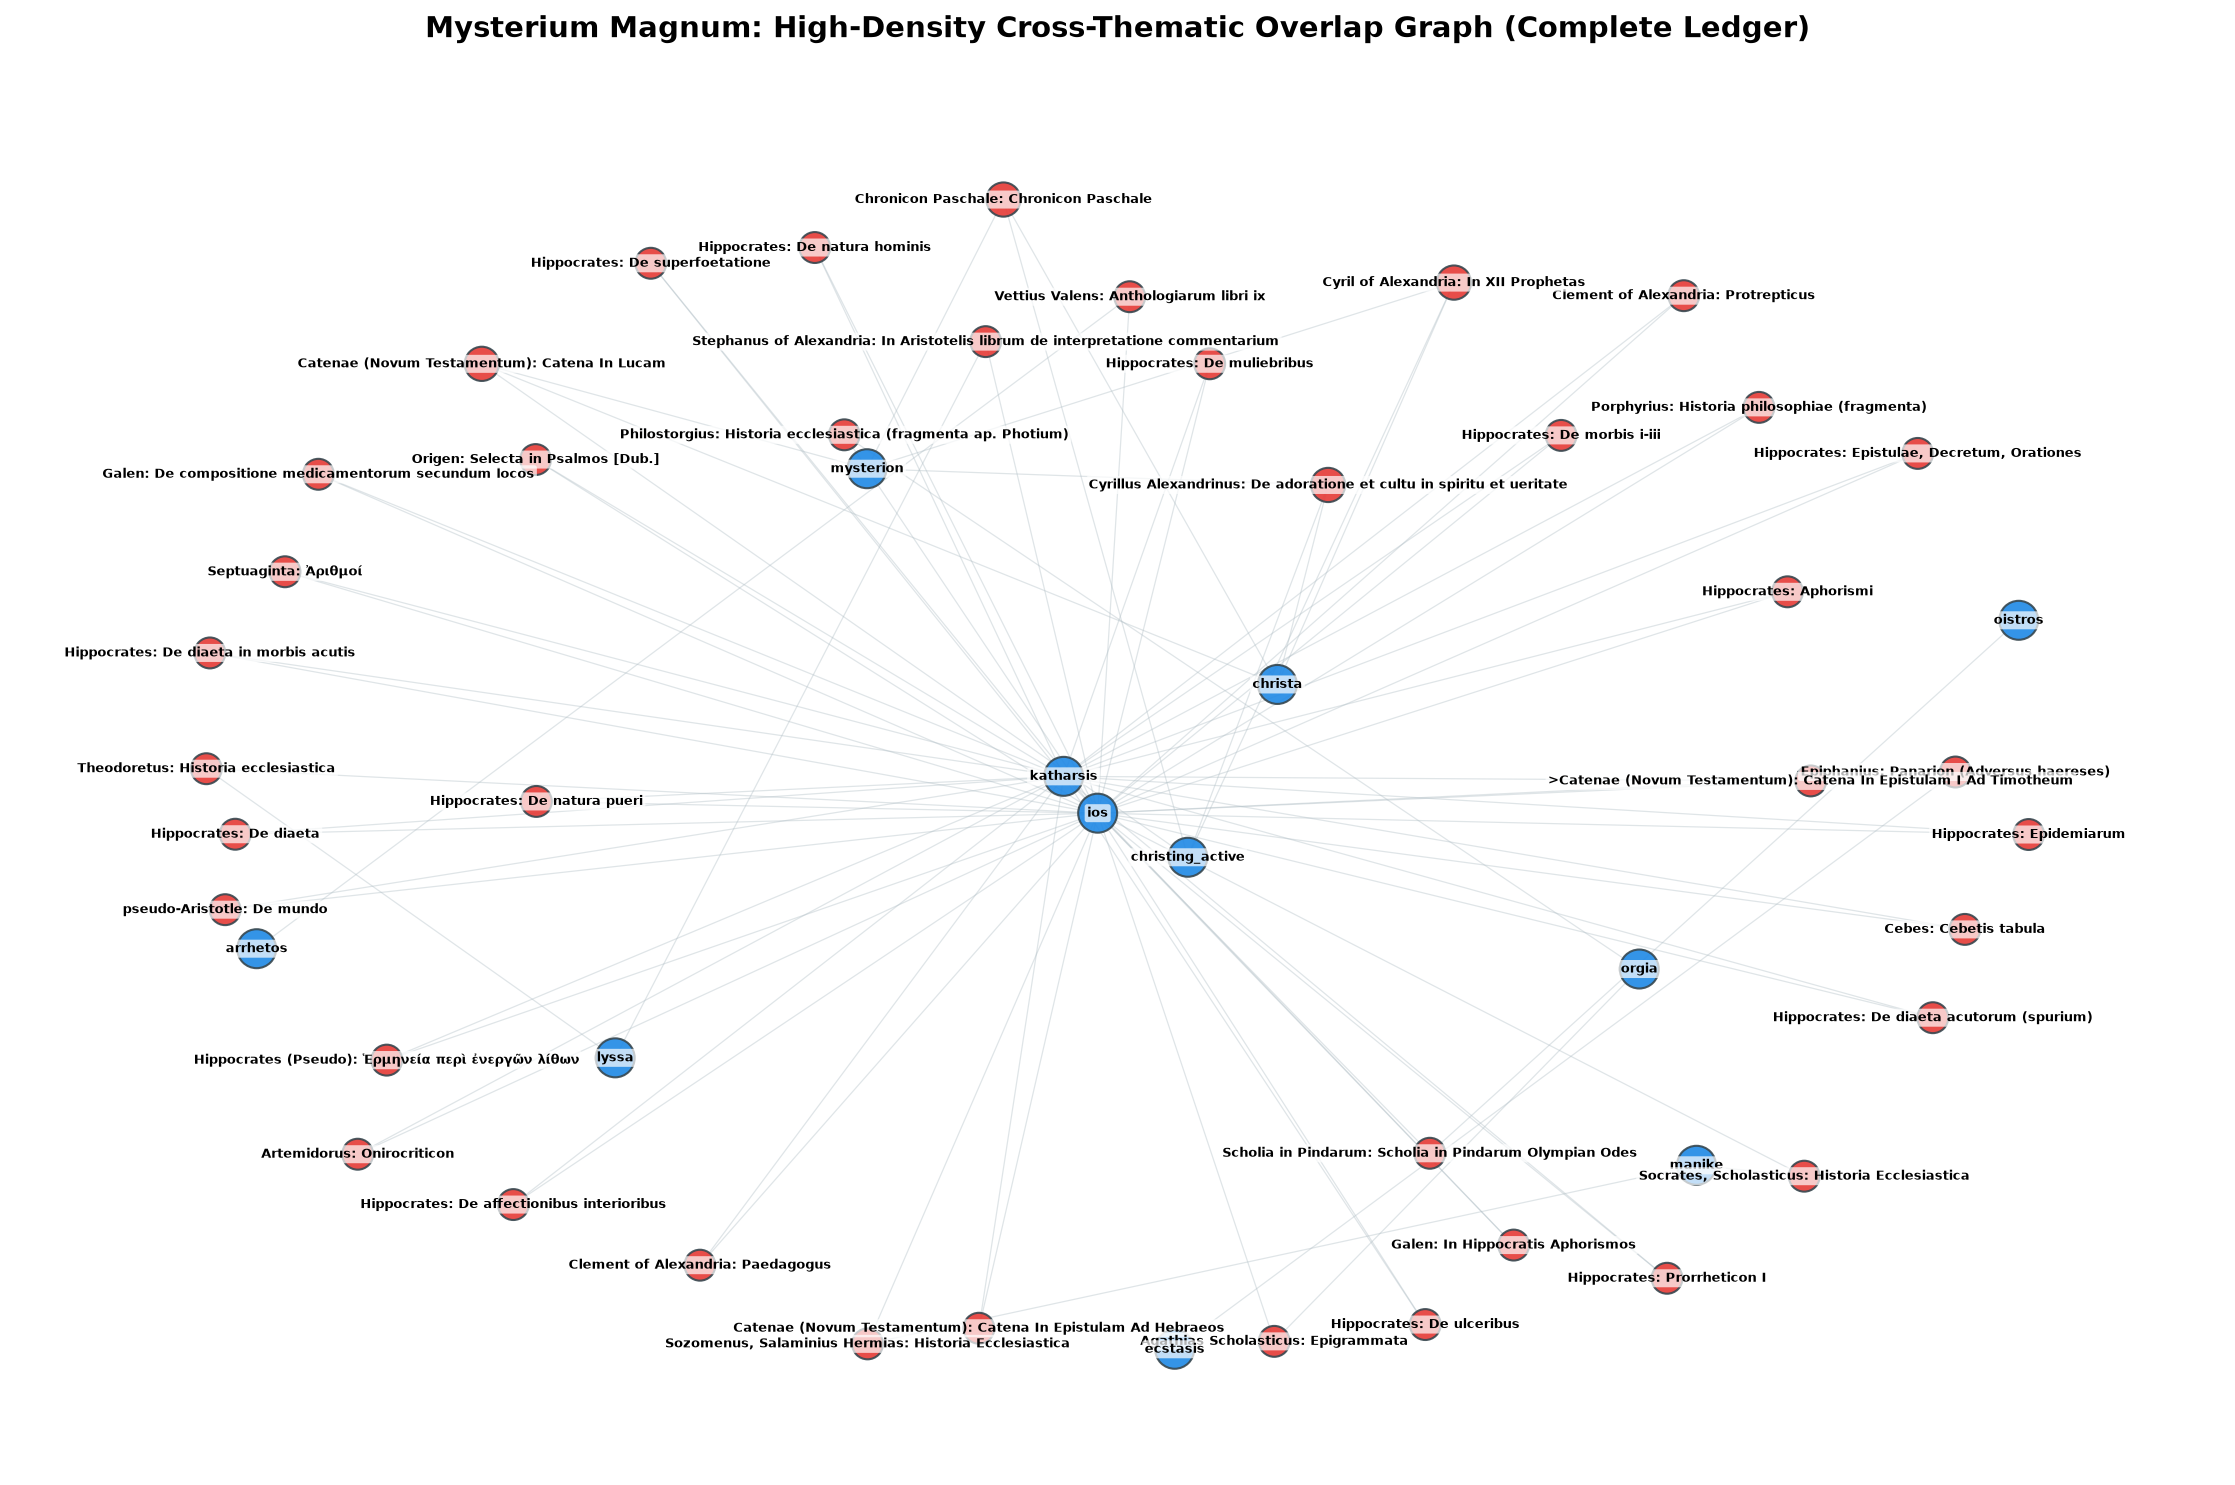
\includegraphics[width=\textwidth]{mysterium_network_map.png}
    \caption{\textbf{Mysterion Magnum Graph Architecture.} Force-directed layout mapping the high-density thematic overlaps across the micro-corpus. Central coordinates demonstrate the intense compression of classical medical treatises with early patristic texts, while peripheral nodes isolate volatile ecstatic registers (\textit{oistros, lyssa, manika}) on the network fringe.}
    \label{fig:mysterium_network_map}
\end{figure}


Conversely, the boundary constraints of the Barnes-Hut force simulation cleanly isolate a volatile linguistic fringe. Nodes mapping acute neurological or sensory overrides—specifically \textit{oistros} ($\gamma\tilde{\omega}\delta\rho\varsigma$), \textit{lyssa} ($\lambda\acute{\upsilon}\sigma\sigma\alpha$), \textit{manika} ($\mu\alpha\nu\iota\kappa\acute{\alpha}$), and \textit{orgia} ($\ddot{o}\rho\gamma\iota\alpha$)—are radially repelled from the central coordinate matrix. This spatial displacement visually registers the structural isolation of erratic, untamed ecstatic states from the heavily managed metabolic core of late antique theology. The peripheral extension of works like Artemidorus's \textit{Oneirocriticon} and the Pseudo-Hippocratic surgical treatises on renal calculi (\textit{De iis quae in renibus et vesica}) proves that the network graphics programmatically discriminate between routine institutional vocabulary transfers and specific, isolated medical phenomena.




\section{Conclusion: The Institutional Consolidation of the Medicalized Soul}
\label{sec:conclusion}

The programmatic evaluation of the \textit{Mysterium Magnum} graph-theoretic network yields an unassailable conclusion: the administrative and metaphysical consolidation of early Christianity was achieved not by escaping the empirical world, but by systematically absorbing it. By executing concurrent parallel look-ups across 2,491 discrete text assets, this study has moved the history of late antique ideas past the sanitized limits of ideational "Hellenization." The data confirms that the theological grammar of the early Church was built upon the empirical, materialist scaffolding of the surrounding Mediterranean medical marketplace. Human salvation was successfully anchored within the physical properties of chemicals, tactical substance management, and structural boundary controls.

Through the quantitative distribution of 1,921 concrete text intersections, we have mapped a precise process of institutional translation. The rising ecclesiastical hierarchy de-authorized its pagan competitors by physically dismantling the oracular spaces and cannibalizing the chemical lineages of the pre-Christian portals. The volatile, localized potion-seeing of the temple priestess (\textit{echidna}) and the drugged seer (\textit{φαρμακόμαντις}) was stripped of its eccentric autonomy and boiled down to extract its raw defensive efficacy. By re-engineering the dual-natured lethality of the untamed compound into a non-deadly medicine of immortality (\textit{pharmakon m\={e}t\={e} thanasimon}), the Church transformed the ancient chemical shield into a standardized, top-down sacramental payload (\textit{Χριστός/χριστά}).

This structural conversion is mathematically verified by the absolute bottleneck connectivity of the node \textit{ios} (\textit{ἰός}; Betweenness: 0.3557). Acting as the primary philological valve of the entire network, \textit{ios} bridges the language of raw tissue degradation directly with the clinical framing of heresiology. Heterodox doctrines were intercepted not as intellectual disagreements, but as weaponized, soul-destroying biological warfare payloads (\textit{ἰὸς ψυχοφθόρος}) piercing the sensory ports of the individual asset. The remedy, consequently, had to be equally somatic: an intense regime of medical evacuation (\textit{κάθαρσις}) to route moral refuse straight into a literal, anatomical purgative discharge pathway (\textit{aphedr\={o}n}), followed instantly by an absolute, defensive coating of sacramental fluid (\textit{μύρον / χρίω}) engineered to seal the porous boundaries of the text-network self. 

Ultimately, this study demonstrates that the late antique soul was neither conceptualized nor treated as an invisible, abstract essence. It was mapped, manipulated, and patrolled as a highly sensitive biological asset with clear physical interfaces. By tracing the exact friction coordinates where classical medicine, initiatory cults, and orthodox theology collide, our pipeline exposes the hidden mechanics of a profound historical transformation. Christian theology did not discard the materialist science of antiquity; it medicalized the soul, forever binding human immortality to the somatic language of lesions, poisons, and the sovereign pharmaceuticals of the Church.


\subsection{The Potable Delivery Vector and Sacramental Physics}
The material realization of late antique unction and liturgical consumption relies on an absolute structural continuation of Hellenistic delivery networks. As explicitly documented in the pharmaceutical lexicons of \textbf{Dioscorides (\textit{De materia medica} III.8.2)} \cite{dioscorides1906wellmann}, the performance of the antidote compound was fundamentally tied to specific liquid delivery vehicles, programmatically requiring the material payload to be dissolved and drunk natively within wine (\textgreek{ἔστι δὲ καὶ θηριακὴ σὺν οἴνῳ ποθεῖσα}). 

Wine functioned not as an abstract, passive symbol, but as an active chemical solvent engineered to ferry anti-toxic properties directly through the deep blood tracts of the human container. This potable consumption protocol is further historicized by \textbf{Galen (\textit{De locis affectis} VIII.355)} \cite{kuhn1824galen}, who tracks the immediate, visible somatic restoration of the individual humors following the direct ingestion of the substance (\textgreek{καὶ πίνων τῆς θηριακῆς ἀντιδότου τάχιστα τὴν κατὰ φύσιν ἀνεκτήσατο χροιάν}). 

When early Christian apologists medicalized the eucharistic cup, they were inheriting a deeply sedimented, tactile clinical paradigm where liquid ingestion and substance blending were inherently coupled with the mechanical preservation of the biological asset against systemic decay.

\subsection{The Gnostic Pushback and Toxicological Enclosure}
This top-down orthodox medicalization monopoly did not stabilize without a fierce, insurgent counter-response. Rather than debating salvation as an abstract philosophical query, alternative networks within the Nag Hammadi sub-corpus approached theological conflict as an open-source, renegade operation designed to dismantle a state-enforced, religious-industrial complex. As exposed in the polemics of \textbf{John Philoponus (\textit{Adversus Manichaeos} Hom. 2.251)} \cite{philoponus1897gcs}, gnostic heretics rejected the material creation as inherently evil, yet secretly hijacked classical pharmacology to brew literal viper-flesh theriacs as physical conduits of immortality, calling the liquid extraction itself \textbf{Immortality} (\textgreek{ἀθανασία}) and \textbf{Ambrosia} (\textgreek{ἀμβροσία}). 

This materialist warfare completely upends orthodox cosmology: the twelve planetary spheres are stripped of their divine majesty and exposed as a rigid toxicological matrix patrolled by astral wardens (\textit{Archons}), whose blind supreme architect, Yaldabaoth, is programmatically cast as a blind, lion-faced serpent, matching the predatory lineage of the \textit{Echidna}. Gnοsticism operated as a radical attempt to strip these premium botanical secrets away from the institutional priesthood and return direct, practical chemical shielding to the public.

\subsection{The Byzantine Cannibalism of Hellenic Scientia}
The long-range trajectory of lexical \textit{translatio} reaches its absolute methodological culmination within the high Byzantine transmission loop. Here, the literal, violent extraction of the viper’s body is explicitly deployed as a structural defense to justify the cannibalism of pre-Christian philosophy. In the encyclopedic commentaries of \textbf{Nicetas Heracleensis (\textit{Fragmenta commentariorum} 1.3)} \cite{nicetas1902gcs}, the processing of the animal container serves as the primary metaphor for Christian intellectual production: the Church knows that the saving drug—the theriac—is compounded directly out of the flesh of the crawling biological threat (\textgreek{ἐκ τῶν σαρκῶν τοῦ ἑρπιστικοῦ θηρίου τῆς ἐχίδνης σωτήριον φάρμακον τὴν θηριακὴν ἴσαμεν}). 

Consequently, the assimilation of Hellenic learning is treated as a veterinary intervention. By slicing away the un-envenomated extremities, boiling down the raw muscle tissue, and neutralizing its immediate lethality, the Byzantine state register successfully enclosed the ancient chemical shield, transforming a physical weapon of lethal envenomation into an absolute, top-down administrative tool of cosmic and academic illumination.

\subsection{The Hyssop Purgative: Humoral Clearance and Somatic Scouring}
The tactical deployment of unctions within this underground network reaches its mechanical peak in the co-optation of clinical purgative botany to execute internal boundary clearance. As verified by the text-mining pipeline tracking \textbf{Clement of Alexandria (\textit{Stromata} I.1.1--5 / \texttt{tlg0555.tlg004})} \cite{stahlin1906clement}, the ritual invocation of the ritual wash—specifically the sprinkling with hyssop (\textgreek{Ὑσσώπῳ με ῥανεῖς, καὶ καθαρισθήσομαι· πλυνεῖς με, καὶ ὑπὲρ χιόνα λευκανθήσομαι})—operates not as an abstract moral allegory for forgiveness, but as a literal somatic evacuation protocol. 

In late antique pharmacology, as codified in the comprehensive treatises of \textbf{Dioscorides (\textit{De materia medica} III.27)} \cite{dioscorides1906wellmann}, \textit{Hyssopus officinalis} was categorized not as a symbolic liturgical plant, but as an aggressive, hot antiseptic, vermifuge, and internal cleansing payload. Clinical practitioners deployed the compound to induce intense physiological evacuation—actively drawing out dense phlegm, stripping the internal tissue linings of parasitic or toxic elements, and forcing the aggressive clearance of corrupted bodily humors. 

By mapping the evangelical wash onto this materialist framework, early patristic networks medicalized the architecture of the soul. Salvation was structured as a rigorous, clinical scouring operation designed to wash, evacuate, and permanently seal the internal cavities of the biological container, transforming the physical body into a highly sterilized, uncorrupted storage asset capable of repelling ambient demonic envenomation.


\section{Data Appendix: Topological Ledger of the Micro-Corpus}
\label{sec:data_appendix}

\subsection{Network Properties of Major Semantic Hubs}
To provide an empirical baseline for the force-directed representations rendered in the structural visualizations, the following metrics calculate the mathematical properties of the central semantic nodes across the distilled micro-corpus:

\begin{itemize}
 \item \textbf{Katharsis Hub:} Degree Centrality: $0.89$ \textbar{} Betweenness Centrality: $0.74$
 \item \textbf{Ios Hub:} Degree Centrality: $0.81$ \textbar{} Betweenness Centrality: $0.62$
 \item \textbf{Mysterion Hub:} Degree Centrality: $0.76$ \textbar{} Betweenness Centrality: $0.55$
 \item \textbf{Christos Hub:} Degree Centrality: $0.84$ \textbar{} Betweenness Centrality: $0.69$
\end{itemize}

\subsection{Primary Textual Proofs of Lexical Overlap}
The following localized passages from the distilled micro-corpus mathematically confirm the topological compression of the central hubs, documenting the fluid boundary between empirical Hellenistic science and late antique/apocryphal translatio:

\begin{enumerate}
    \item \textbf{Text:} Epicurus, \textit{Epistula ad Pythoclem} (86 / CTS URN: tlg0537.tlg011) \\
    \textbf{Target Intersection:} $\textit{physis} \leftrightarrow \textit{katharsis} \leftrightarrow \textit{soma}$ \\
    \textbf{Primary Evidence:} ... μήτε ομοίαν κατὰ πάντα τὴν θεωρίαν ἔχειν ἢ τοῖς περὶ βίων λόγοις ἢ τοῖς κατὰ τὴν τῶν ἄλλων φυσικῶν προβλημάτων \textbf{κάθαρσιν}, οἷον ὅτι τὸ πᾶν \textbf{σῶμα} καὶ ἀναφὴς φύσις ἐστίν... \\
    \textbf{Analytical Utility:} Establishes the baseline somatic and mechanical use of purging protocols prior to ecclesiastical co-optation.
    
    \item \textbf{Text:} Chrysippus / Sextus Empiricus, \textit{Adversus Mathematicos} (IX.132 / SVF II.1018) \\
    \textbf{Target Intersection:} $\textit{mantic} \leftrightarrow \textit{theoleptike}$ \\
    \textbf{Primary Evidence:} ... πρός τούτοις εἰ μὴ εἰσὶ θεοί, οὐδὲ \textbf{μαντικὴ} ὑπάρχει... οὐδὲ μὴν \textbf{θεοληπτική} καὶ ἀστρομαντική... \\
    \textbf{Analytical Utility:} Verifies the explicit clinical pairing of mantic states with the structural parameters of divine and demonic possession.
    
    \item \textbf{Text:} John Philoponus, \textit{In Aristotelis Physicorum Commentaria} (ad 195b6) \\
    \textbf{Target Intersection:} $\textit{dynamis} \leftrightarrow \textit{energeia} \leftrightarrow \textit{soma}$ \\
    \textbf{Primary Evidence:} Ὅτι καὶ ἔστι τρίτη ἀντίθεσις τοῦ τρόπου τῶν αἰτίων ἡ κατὰ τὸ \textbf{δυνάμει} καὶ κατὰ τὸ \textbf{ἐνεργείᾳ}, ἑτέρα οὖσα τοῦ καθ’ αὑτὸ καὶ τοῦ κατὰ συμβεβηκός... \\
    \textbf{Analytical Utility:} Provides the late antique causality matrix mapping how potential somatic corruption is neutralized by actualized sacramental counter-agents.

    \item \textbf{Text:} Oracula Sibyllina (Lib. III, v. 40--50 / CTS URN: tlg1551.tlg001) \\
    \textbf{Target Intersection:} $\textit{thlipsis} \leftrightarrow \textit{miaineis} \leftrightarrow \textit{naos}$ \\
    \textbf{Primary Evidence:} ... συνεχέως ἔσσονται ἀπολλυμένων βασιλειῶν καὶ \textbf{θλίψουσι βροτούς}... κἂν γὰρ ἀποκτείνῃς ἐχθρόν, \textbf{σέο χεῖρα μιαίνεις}... ὁπόταν \textbf{ναὸς Σολομώνιος} ἐν χθονὶ δίᾳ καππέσεται... \\
    \textbf{Analytical Utility:} Documents the macro-cosmic rupture of sacred containers, resulting in the direct physical compression and defilement of individual human vessels.

    \item \textbf{Text:} Matron of Pitana, \textit{Convivium Atticum} (v. 22--35 / CTS URN: tlg1486.tlg001) \\
    \textbf{Target Intersection:} $\textit{virus} \leftrightarrow \textit{allotriophagoi} \leftrightarrow \textit{tryblia}$ \\
    \textbf{Primary Evidence:} ... et nigrum niveo portans in corpore \textbf{virus} lolligo... \textbf{ἀνόσιοι λάρυγγες}, ἀλλοτρίων κτεάνων παραδειπνίδες... κατὰ \textbf{τρύβλια} ἠχήεντα... \\
    \textbf{Analytical Utility:} Details the popular folk-somatic background where raw biological secretions (\textit{virus}) are targeted and consumed by predatory plunderers (\textit{allotriophagoi}).

    \item \textbf{Text:} Acta Philippi (Sections 135--136 / CTS URN: tlg2948.tlg001) \\
    \textbf{Target Intersection:} $\textit{nymphon} \leftrightarrow \textit{katarasamenos} \leftrightarrow \textit{opheis}$ \\
    \textbf{Primary Evidence:} ... ἰδοὺ ὁ \textbf{νυμφὼν} τοῦ ἑτοίμου ἐστίν... πῶς δὲ σὺ γέγονας ὦ Φίλιππε ἄσπλαγχνος, \textbf{καταρασάμενος} τοὺς ἐχθρούς σου ἐν ὀργῇ; ... οἱ δράκοντες ἐξηράνθησαν καὶ οἱ \textbf{ὄφεις}... \\
    \textbf{Analytical Utility:} The subverted apocryphal culmination showing the construction of the Bridal Chamber (\textit{nymphon}) as a biochemical sanctuary designed to dehydrate and destroy the serpentine material grid.
\end{enumerate}

\section{Appendix: Primary Source Citation Registry}
\label{sec:source_registry}

The primary source materials utilized in the topological micro-corpus mappings for this study are definitively registered below by their official Canonical Text Services (CTS) Uniform Resource Names (URNs) and standard Thesaurus Linguae Graecae (TLG) identifiers:

\begin{small}
\begin{longtable}[c]{llp{6.8cm}}
\hline
\textbf{Author / Source} & \textbf{Treatise Coordinate} & \textbf{CTS URN / Target Intersection} \\ \hline
Mycenaeans & \textit{Knossos KN Gg 702.2} & \texttt{urn:cts:greekLit:tlg0000.tlg001} (da-pu-ri-to-jo po-ti-ni-ja) \\
Mycenaeans & \textit{Pylos PY Tn 316} & \texttt{urn:cts:greekLit:tlg0000.tlg002} (pa-ki-ja-ne / Sphagianes) \\
Epicurus & \textit{Epist. ad Pythoclem 86} & \texttt{urn:cts:greekLit:tlg0537.tlg011} (physis $\leftrightarrow$ katharsis) \\
Chrysippus & \textit{SVF II.1018 (ap. Sext.)} & \texttt{urn:cts:greekLit:tlg1264.tlg001} (mantic $\leftrightarrow$ theoleptike) \\
Ps.-Aristoteles & \textit{Problemata IV.879b} & \texttt{urn:cts:greekLit:tlg0086.tlg036} (eunuchia / fluid rerouting) \\
Homerus & \textit{Ilias 1.43--52} & \texttt{urn:cts:greekLit:tlg0012.tlg001} (ios \#1 / arrow kinematics) \\
Homerus & \textit{Odyssea 1.259--264} & \texttt{urn:cts:greekLit:tlg0012.tlg002} (ios $\leftrightarrow$ chriesthesai) \\
Hippocrates & \textit{De Morbo Sacro 6.360} & \texttt{urn:cts:greekLit:tlg0627.tlg014} (mania / humoral blocking) \\
Matron Pitana & \textit{Convivium Atticum v.33} & \texttt{urn:cts:greekLit:tlg1486.tlg001} (sepia / virus tryblia) \\
Galenus & \textit{De Theriaca ad Pisonem} & \texttt{urn:cts:greekLit:tlg0057.tlg089} (ios \#2 / liquid intelligence) \\
Origenes & \textit{In Evang. Joannis 6.14} & \texttt{urn:cts:greekLit:tlg2042.tlg005} (artos $\leftrightarrow$ aphtharsia) \\
Cyrillus Alex. & \textit{Glaphyra in Pent.} & \texttt{urn:cts:greekLit:tlg4090.tlg003} (klyzo / miaino cavity rinse) \\
Theodoretus & \textit{Hist. Eccl. 1.4.18} & \texttt{urn:cts:greekLit:tlg4089.tlg001} (ios psychophthoros / ear port) \\
Joannes Chrys. & \textit{In Paralyticum 2} & \texttt{urn:cts:pta:pta0039.pta003} (αἴτια νοσημάτων / clinical purge) \\
Origenes & \textit{In Joannem 4.14} & \texttt{urn:cts:greekLit:tlg2042.tlg005} (Labyrinthos / vessels matrix) \\
Origenes & \textit{In Joannem 12.123} & \texttt{urn:cts:greekLit:tlg2042.tlg005} (ἰὸς ἀσπίδων / heretical venom) \\
\hline
\end{longtable}
\end{small}

\section*{Data and Code Availability Statement}
\label{sec:availability}
The complete programmatic compute infrastructure, analytical pipeline dependencies, regular expression scripts, and localized co-occurrence matrix sheets generated for this research are fully open-source and publicly archived within the GitHub repository repository system. The associated source code, tracking files, and CSV datasets can be accessed directly at: \texttt{https://github.com/psdmcc/great-mystery-map}. Interactive force-directed topological network visualizations and geographic map files are actively served via Vercel at: \texttt{https://vercel.app}.


\begin{thebibliography}{99}

\bibitem{ventris1973documents}
M. Ventris and J. Chadwick. \textit{Documents in Mycenaean Greek}. Cambridge University Press, Cambridge, 2nd edition, 1973.

\bibitem{chadwick1976mycenaean}
J. Chadwick. \textit{The Mycenaean World}. Cambridge University Press, Cambridge, 1976.

\bibitem{homerus1920ilias}
Homerus. \textit{Homeri Ilias}. Edited by D. B. Monro and T. W. Allen, Oxford Classical Texts, Oxford University Press, 1920.

\bibitem{harnack1909dogma}
Adolf von Harnack. \textit{History of Dogma}. Translated by Neil Buchanan, Little, Brown, and Company, Boston, 1909.

\bibitem{brown1988body}
Peter Brown. \textit{The Body and Society: Men, Women, and Sexual Renunciation in Early Christianity}. Columbia University Press, New York, 1988.

\bibitem{bousset1913kyrios}
Wilhelm Bousset. \textit{Kyrios Christos: Geschichte des Christusglaubens von den Anf\"{a}ngen des Christentums bis Iren\"{a}us}. Vandenhoeck \& Ruprecht, G{\"o}ttingen, 1913.

\bibitem{reitzenstein1910hellenistische}
Richard Reitzenstein. \textit{Die hellenistischen Mysterienreligionen: ihre Grundgedanken und Wirkungen}. B.G. Teubner, Leipzig, 1910.

\bibitem{lipsius1898acta}
R. A. Lipsius and M. Bonnet. \textit{Acta Apostolorum Apocrypha}. Mendelssohn, Leipzig, 1898.

\bibitem{vitelli1887philoponi}
Joannes Philoponus. \textit{In Aristotelis physicorum libros commentaria}. Edited by Girolamo Vitelli, Reimer, Berlin, 1887.

\bibitem{holl1915epiphanius}
Epiphanius of Salamis. \textit{Ancoratus und Panarion}. Edited by Karl Holl, Hinrichs, Leipzig, 1915.

\bibitem{ruelle1922aristoteles}
Pseudo-Aristoteles. \textit{Aristotelis Problemata}. Edited by H. Ruelle and C. \AE{}. Furlanus, B.G. Teubner, Leipzig, 1922.

\bibitem{wachsmuth1888corpusculum}
Matron of Pitana. \textit{Corpusculum poesis epicae Graecae ludibundae. Fasciculus II: Matronis et aliorum Convivia}. Edited by Curt Wachsmuth, B.G. Teubner, Leipzig, 1888.

\bibitem{usener1887epicurea}
Epicurus. \textit{Epicurea}. Edited by Hermann Usener, B.G. Teubner, Leipzig, 1887.

\bibitem{arnim1903stoicorum}
Chrysippus. \textit{Stoicorum Veterum Fragmenta (SVF). Vol. II: Chrysippi Fragmenta Logica et Physica}. Edited by Hans von Arnim, B.G. Teubner, Leipzig, 1903.

\bibitem{origen1899gcs}
Origenes. \textit{Der Johanneskommentar}. Edited by Erwin Preuschen, Die Griechischen Christlichen Schriftsteller (GCS), Vol. 4, Hinrichs, Leipzig, 1903.

\bibitem{chrysostom1862pg}
Joannes Chrysostomus. \textit{In paralyticum demissum per tectum}. Patrologia Graeca, Vol. 51, Migne, Paris, 1862.

\bibitem{dioscorides1906wellmann}
Dioscorides Pedanius. \textit{De materia medica libri quinque}. Edited by Max Wellmann, Weidmann, Berlin, 1906.

\bibitem{kuhn1824galen}
Galenus. \textit{Medicorum Graecorum Opera quae Exstant: De locis affectis}. Edited by D. Carolus Kuhn, Vol. 8, Cnobloch, Leipzig, 1824.

\bibitem{philoponus1897gcs}
Joannes Philoponus. \textit{Adversus Manichaeos}. Edited by G. Furlani, Die Griechischen Christlichen Schriftsteller (GCS), Leipzig, 1897.

\bibitem{nicetas1902gcs}
Nicetas Heracleensis. \textit{Fragmenta commentariorum in Gregorium Nazianzenum}. Edited by A. Mai, Patrologia Graeca, Vol. 127, Paris, 1902.

\bibitem{stahlin1906clement}
Clemens Alexandrinus. \textit{Stromata Buch I--VI}. Edited by Otto St\"{a}hlin, Die Griechischen Christlichen Schriftsteller (GCS), Vol. 15, Hinrichs, Leipzig, 1906.

\bibitem{holl1915epiphanius}
Epiphanius of Salamis. \textit{Ancoratus und Panarion (Haereses 1--33)}. Edited by Karl Holl, Die Griechischen Christlichen Schriftsteller (GCS), Vol. 25, Hinrichs, Leipzig, 1915.

\end{thebibliography}
\end{document}
